\documentclass{ximera}

\title{How to use Ximera}

\begin{document}
\begin{abstract}
  This course is built in Ximera.
\end{abstract}\maketitle

Mathematics cannot be learned passively: it must be actively
\link[constructed]{http://en.wikipedia.org/wiki/Constructivism_(philosophy_of_education)}
by the person learning it.  With this in mind, this course is built
around solving problems!

Here are some examples.  Play around with it, get it wrong, try the
hints out.  Don't be afraid to fail: \textbf{getting an answer wrong
  never hurts you.}


\begin{example}
  Some problems are multiple-choice:
  \begin{multipleChoice}
    \choice{Don't pick me.}
    \choice{Not me either.}
    \choice[correct]{Pick me!}
    \choice{Also an incorrect choice}
  \end{multipleChoice}
  \begin{feedback}
    Click on the choice that says ``Pick me!''
  \end{feedback}
\end{example}


\begin{example}
  Some problems are select-all that are correct:
  \begin{selectAll}
    \choice{Don't pick me.}
    \choice[correct]{Pick me!}
    \choice[correct]{Pick me too!}
    \choice[correct]{I'm a correct choice too.}
  \end{selectAll}
  \begin{feedback}
    Click on the choices ``Pick me!'' ``Pick me too!'' and ``I'm a correct choice too.''
  \end{feedback}
\end{example}


\begin{example}
Some problems are fill in the blank: 
  $3\times 2 = \answer{6}$   
  \begin{hint}
    $3 \times 2$ is the number of objects in $3$ groups of $2$ objects
  \end{hint}
  \begin{hint}
    \begin{image}
      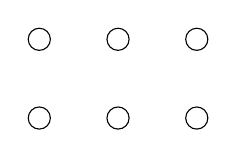
\begin{tikzpicture}
        \draw (0,0) circle (4pt);
        \draw (1,0) circle (4pt);
        \draw (2,0) circle (4pt);
        \draw (0,1) circle (4pt);
        \draw (1,1) circle (4pt);
        \draw (2,1) circle (4pt);
      \end{tikzpicture}
    \end{image}
  \end{hint}
  \begin{hint}
    $3\times 2=6$
  \end{hint}
\end{example}

For this course, you should always have a paper and pencil near at
hand to make notes, doodle pictures, or solve complicated equations.
We \textbf{strongly} recommend that you really \textbf{grapple} with a
problem before getting a hint, or moving on.  The difference between
what you learn by struggling with a problem on your own versus
perusing someone else's solution is astonishing.

With that said, even if you get an answer right you should
\textbf{always} try the hints out afterwards.  They might explain the
concept from a new point of view, or challenge you to think in a
different way than you solved the problem.


Many fill-in-the-blank problems expect algebraic expressions for answers.  In the examples below, try to retype the expression to the left of the equals sign: 

\begin{example}
  $\frac{x^2+y^2}{7} = \answer{\frac{x^2+y^2}{7}}$
  \begin{feedback}
    Type $\verb|(x^2+y^2)/7|$
  \end{feedback}
\end{example}

\begin{example}
  $\frac{\tan(x)}{2xa+b^2} = \answer{\frac{\tan(x)}{2xa+b^2} }$
  \begin{feedback}
    Type $\verb|tan(x)/(2xa+b^2)|$
  \end{feedback}
\end{example}

\begin{example}
  $\arcsin(x) = \answer{\arcsin(x)}$
  \begin{feedback}
    Type $\verb|arcsin(x)|$

    Note that typing $\verb|sin^(-1)(x)|$ does not work.
  \end{feedback}
\end{example}

\begin{example}
  $|x| = \answer{|x|}$
  \begin{feedback}
    You can type $\verb! |x| !$ or $\verb! abs(x)!$, but
    $\verb! abs(x) !$ may be preferable because it is easier to parse
    appropriately.
  \end{feedback}
\end{example}
\begin{example}
  $\ln(x+1)= \answer{\ln(x+1)}$
  \begin{feedback}
    You could type $\verb|ln(x+1)|$ or $\verb|log(x+1)|$
  \end{feedback}
\end{example}

\begin{example}
  $ \sin(\theta) = \answer{\sin(\theta)}$
  \begin{feedback}
    Type $\verb|sin(theta)|$
  \end{feedback}
\end{example}


\begin{example}
  $ \varphi = \answer{\varphi}$
  \begin{feedback}
    Type $\verb|phi|$
  \end{feedback}
\end{example}


\begin{example}
  $ \rho = \answer{\rho}$
  \begin{feedback}
    Type $\verb|rho|$
  \end{feedback}
\end{example}

\begin{example}
	$\sqrt{x} = \answer{\sqrt{x}}$
  \begin{feedback}
    Type $\verb|sqrt(x)|$
  \end{feedback}
  \begin{feedback}
    It would also work to type $\verb| x^(1/2)|$
  \end{feedback}
\end{example}

\begin{example}
  $\sqrt[3]{y} = \answer{y^{\frac{1}{3}}}$
  \begin{feedback}
    We do not have a ``slick" way to enter this, so you should just
    type $\verb!y^(1/3)!$, which is equivalent.
  \end{feedback}
\end{example}


\begin{example}
  $DNE = \answer[format=string]{DNE}$
  \begin{feedback}
    Type $\verb|DNE|$, which means ``Does Not Exist.''
  \end{feedback}
\end{example}

\begin{example}
  $\infty = \answer{\infty}$
  \begin{feedback}
    Type $\verb|infty|$ or $\verb|infinity|$ or $\verb|oo|$.
  \end{feedback}
\end{example}

As you complete activities the green ``completion bar'' moves at the
top of the page.  This lets you know how close you are to being done
with an activity.

You advance through pages either by completing them and clicking the
``next activity'' button, or by navigating on the little scroll bar at
the top of the page.
 

\end{document}
